% ch3p10_004: Connecting nodes
% "to" operation with "in" and "out" options
\documentclass[tikz, border=10pt]{standalone}

\usepackage{tikz}
\usetikzlibrary{arrows.meta, decorations.pathmorphing, backgrounds, positioning, fit, petri}

\begin{document}
	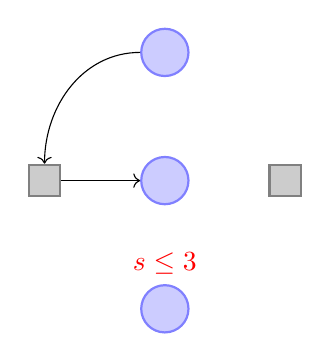
\begin{tikzpicture}[
		place/.style={circle, draw=blue!50, fill=blue!20, thick, inner sep=0pt, minimum size=6mm},
		transition/.style={rectangle, draw=black!50, fill=black!20, thick, inner sep=0pt, minimum size=4mm},
		every label/.style={red}
		]
		\node [place] (waiting) {};
		\node [place] (critical) [below=of waiting] {};
		\node [place] (semaphore) [below=of critical, label=above:$s\le 3$] {};
		\node [transition] (leave critical) [right=of critical] {};
		\node [transition] (enter critical) [left=of critical] {};
		
		\draw [->] (enter critical) to (critical);
		\draw [->] (waiting) to [out=180, in=90] (enter critical);
	\end{tikzpicture}
\end{document}